\documentclass{article}
\usepackage{tikz}
\usetikzlibrary{decorations.text}

\begin{document}

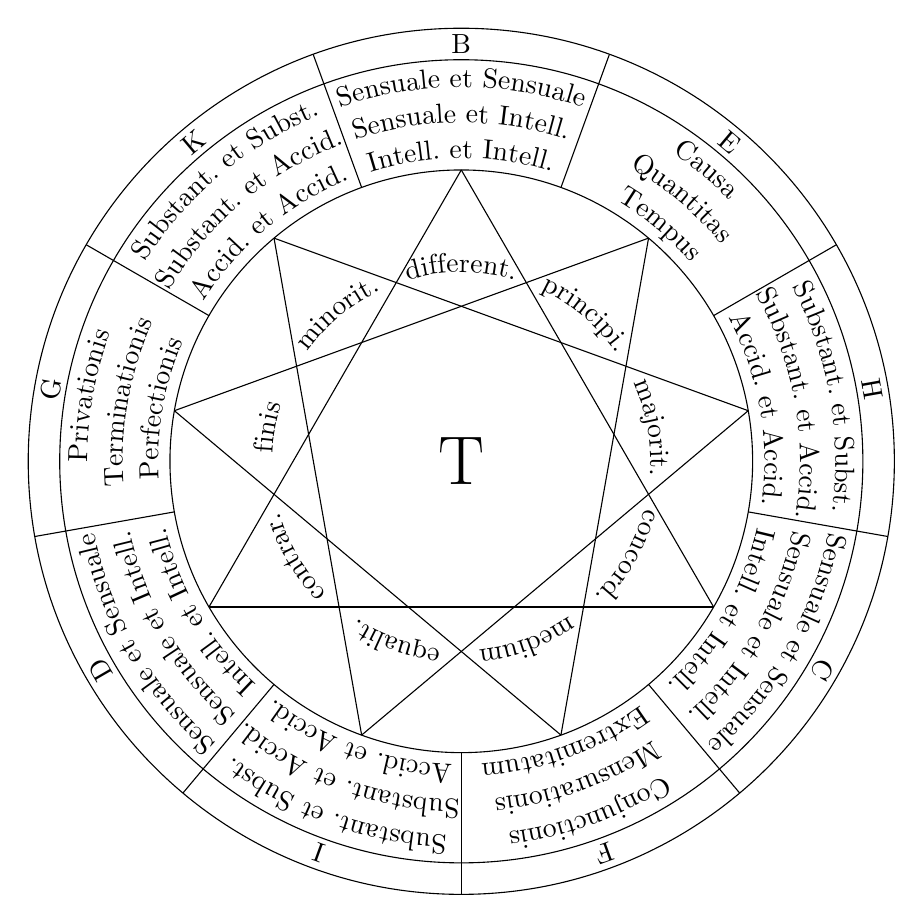
\begin{tikzpicture}

\draw (0,0) node {\Huge{T}}; % Central T

% Rings
\foreach \r in {3.7,5.1,5.5}
  \draw (0,0) circle [radius=\r cm];

% Rays
\foreach \x in {0,...,8}
  \draw (270+40*\x:3.7cm) -- (270+40*\x:5.5cm);

% Rings of Text
\foreach \y in {0,1,2} %
  \foreach \x in {0,...,8} {

    \pgfmathparse{{{"Accid. et Accid.","Intell. et Intell.","Perfectionis","Accid. et Accid.","Intell. et Intell.","Tempus","Accid. et Accid.","Intell. et Intell.","Extremitatum"},
                   {"Substant. et Accid.","Sensuale et Intell.","Terminationis","Substant. et Accid.","Sensuale et Intell.","Quantitas","Substant. et Accid.","Sensuale et Intell.","Mensurationis"},
                   {"Substant. et Subst.","Sensuale et Sensuale","Privationis","Substant. et Subst.","Sensuale et Sensuale","Causa","Substant. et Subst.","Sensuale et Sensuale","Conjunctionis"}}[\y][\x]}
    \edef\letter{\pgfmathresult}


    \draw [decoration={
            text along path,
            text={\letter},
            text align={center}
           },
           decorate]

      (270-40*\x:3.85cm+0.45cm*\y) % Start Location

      arc[start angle=270-40*\x,
          delta angle=-40,
          radius=3.85cm+0.45cm*\y];
}

% Ring of Letters
\foreach \x in {0,...,8} {

    \pgfmathparse{{"I","D","G","K","B","E","H","C","F"}[\x]}
    \edef\letter{\pgfmathresult}

    \draw [decoration={
            text along path,
            text={\letter},
            text align={center}
           },
           decorate]

      (270-40*\x:5.175cm) % Start Location

      arc[start angle=270-40*\x,
          delta angle=-40,
          radius=5.175cm];
}

% Ring of Relations

\foreach \x in {0,...,8} {

    \pgfmathparse{{"equalit.","contrar.","finis","minorit.","different.","principi.","majorit.","concord.","medium"}[\x]}
    \edef\letter{\pgfmathresult}

    \draw [decoration={
            text along path,
            text={\letter},
            text align={center}
           },
           decorate]

      (270-40*\x:2.4cm) % Start Location

      arc[start angle=270-40*\x,
          delta angle=-40,
          radius=2.4cm];
}

% Triangles
\foreach \startdeg in {290, 290+40, 290+40*2}
  \foreach \x in {0,3,6}
    \draw (\startdeg+40*\x:3.7cm) -- (\startdeg+40*3+40*\x:3.7cm);

\end{tikzpicture}

\end{document}
